\begin{frame}
    \centering
    \Huge{Sistemas Operativos Libres}
\end{frame}

\begin{frame}{Sistemas Operativos Libres}
    \begin{itemize}
        \item Android (2008-)
        \pause
        \item Tizen (2013-)
        \pause
        \item KDE Plasma (2015-)
        \pause
        \item Jolla's SailfishOS (2014-)
            \pause
            \begin{itemize}
                \item MeeGo/Maemo/Moblin spiritual successor
            \end{itemize}
            \pause
        \item Ubuntu Touch (2011-2016)
    \end{itemize}
\end{frame}

\begin{frame}
    \centering
    \Huge{¿Es Android realmente libre?}
\end{frame}

\begin{frame}{¿Es Android realmente libre?}
    \textbf{Android is about freedom and choice.\\
				The purpose of Android is to promote openness in the mobile world, and we don't believe it's possible to predict or dictate all the uses to which people will want to put our software.\\
				So, while we encourage everyone to make devices that are open and modifiable, we don't believe it is our place to force them to do so.
    }
    \url{https://source.android.com}
\end{frame}

\begin{frame}{Anatomía de Android}
    \centering
    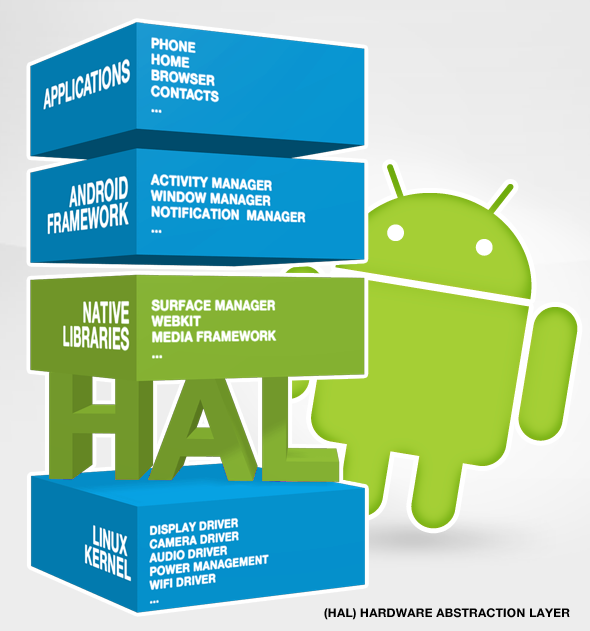
\includegraphics[height=0.7\textheight]{images/android-arch-2.png}
\end{frame}

\begin{frame}{Android Custom ROMs}
    \begin{itemize}
        \item LineageOS, former CyanogenMod (2009-)
        \item Paranoid Android (2012-)
        \item SlimRoms, DirtyUnicorns, Carbon, Resurrection Remix...
    \end{itemize}
\end{frame}

\begin{frame}{Futuro de los SO Libres}
    \centering
    \Huge{¿Fuchsia?}
    
\includegraphics[width=\textwidth]{images/fuchsia.png}
\end{frame}

\begin{frame}{Fuchsia}
    \centering
    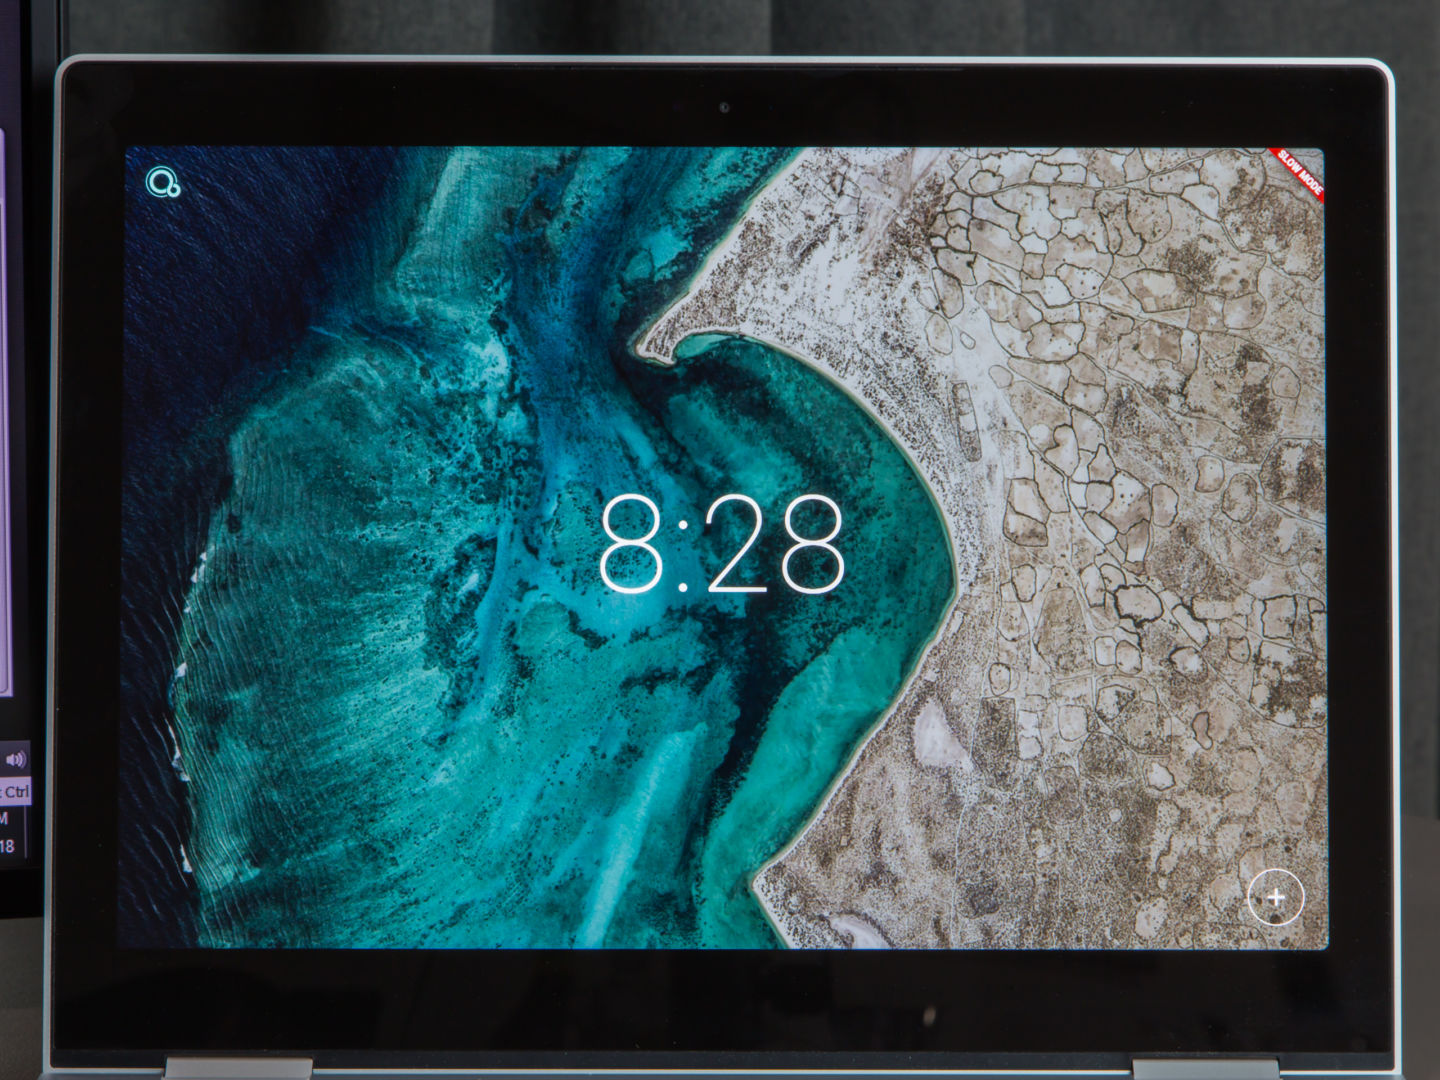
\includegraphics[height=0.7\textheight]{images/fuchsia-1.jpg}
\end{frame}

\begin{frame}{Fuchsia}
    \centering
    \Huge{¿Fuchsia?} \\
    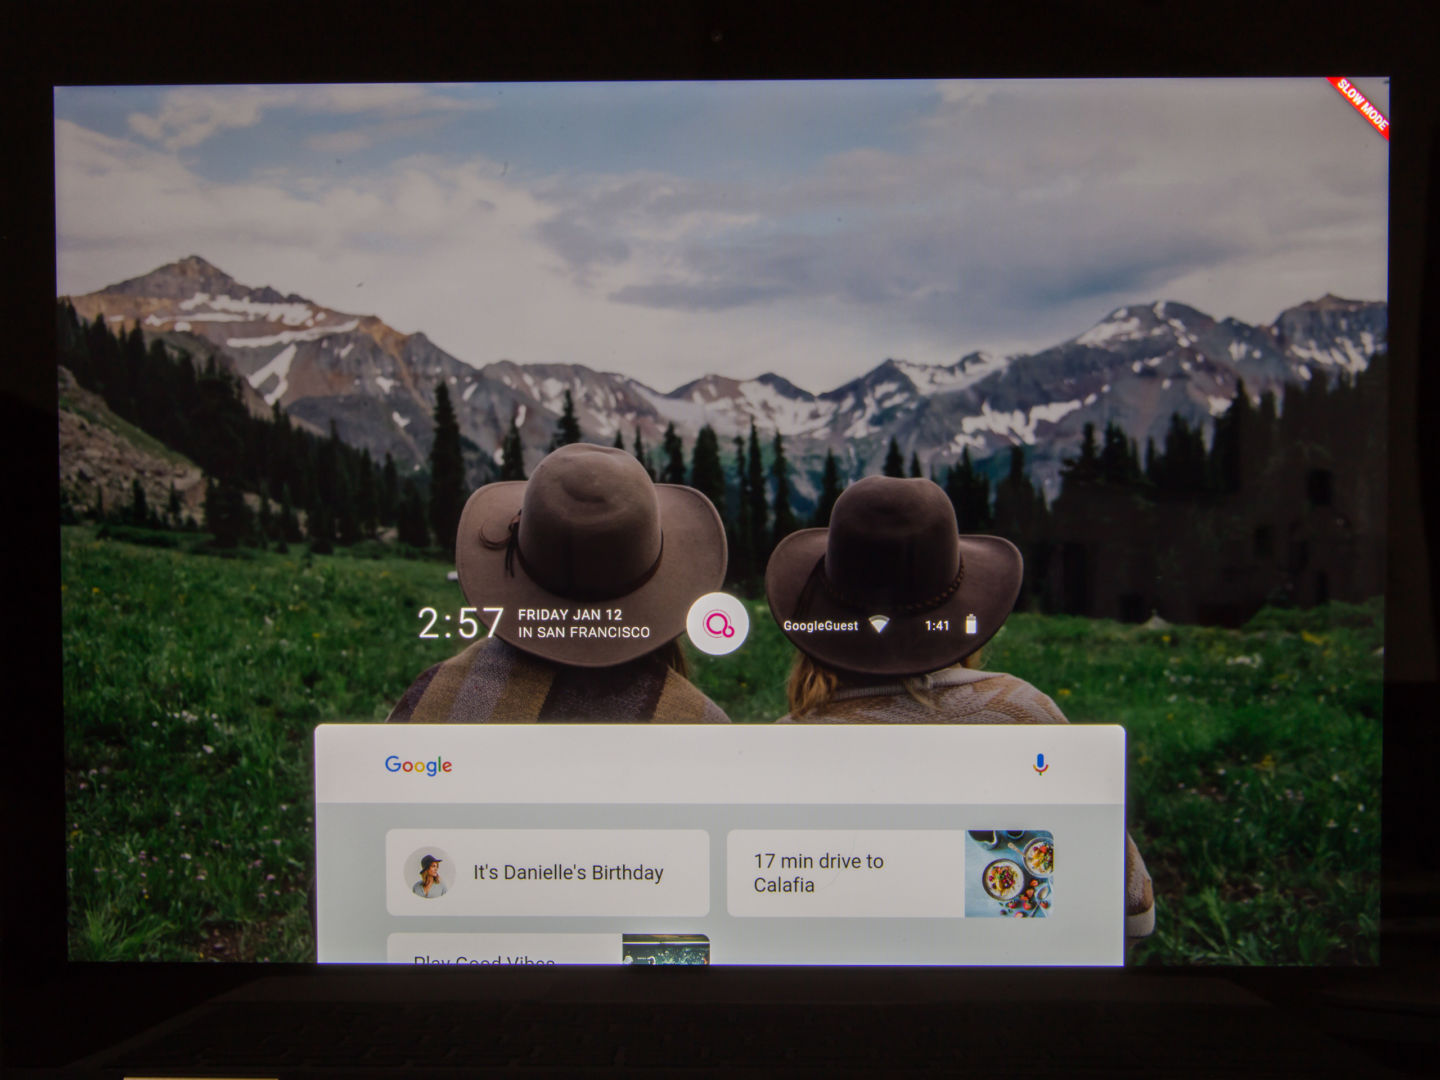
\includegraphics[height=0.7\textheight]{images/fuchsia-2.jpg}
\end{frame}

\begin{frame}{Fuchsia}
    \centering
    \Huge{¿Fuchsia?} \\
    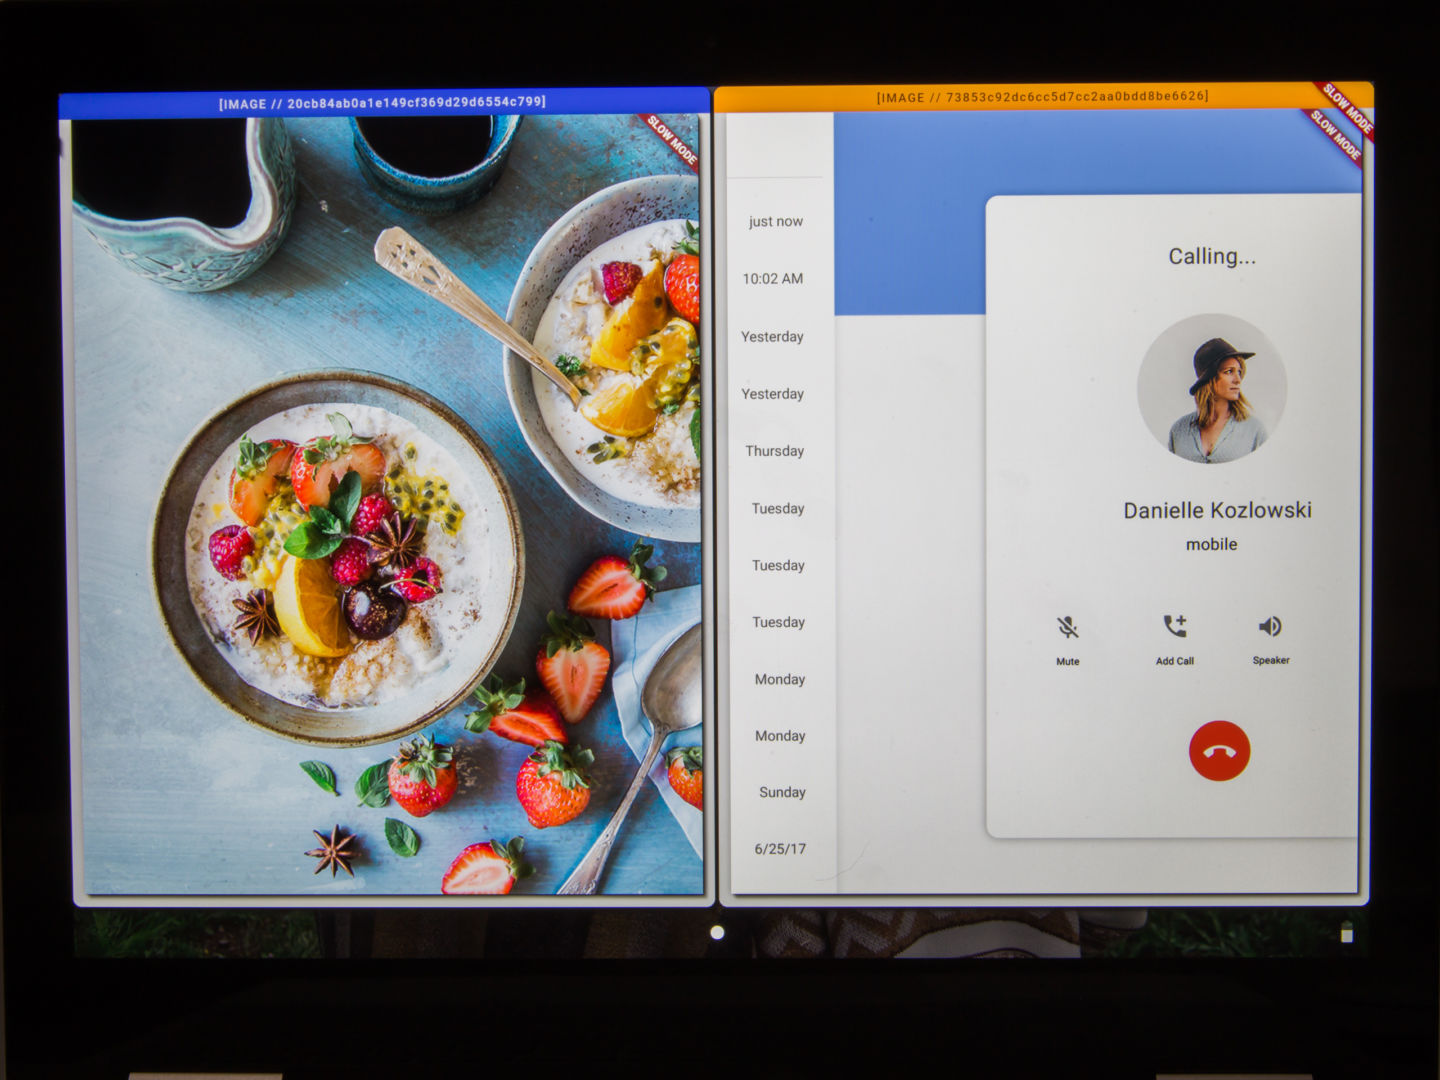
\includegraphics[height=0.7\textheight]{images/fuchsia-3.jpg}
\end{frame}
